\documentclass[11pt,a4paper]{article}
\usepackage[utf8]{inputenc}
\usepackage[T1]{fontenc}
\usepackage{amsmath,amssymb,amsthm}
\usepackage{mathtools}
\usepackage{geometry}
\usepackage{hyperref}
\usepackage{cleveref}
\usepackage{booktabs}
\usepackage{array}
\usepackage{longtable}
\usepackage{tikz}
\usetikzlibrary{arrows.meta,positioning,shapes.geometric,calc,decorations.pathreplacing}
\usepackage{tcolorbox}
\tcbuselibrary{theorems,skins,breakable}
\usepackage{xcolor}
\usepackage{enumitem}

\geometry{margin=1in}

\hypersetup{
    colorlinks=true,
    linkcolor=blue!70!black,
    citecolor=green!50!black,
    urlcolor=blue!70!black
}

% Theorem environments
\newtheorem{theorem}{Theorem}[section]
\newtheorem{lemma}[theorem]{Lemma}
\newtheorem{proposition}[theorem]{Proposition}
\newtheorem{corollary}[theorem]{Corollary}
\newtheorem{definition}[theorem]{Definition}
\newtheorem{remark}[theorem]{Remark}

% Boxes
\newtcolorbox{resultbox}[1][]{
    colback=blue!5!white,
    colframe=blue!75!black,
    fonttitle=\bfseries,
    title=#1,
    breakable
}

\newtcolorbox{selectorbox}[1][]{
    colback=green!5!white,
    colframe=green!60!black,
    fonttitle=\bfseries,
    title=Selector,
    breakable
}

\newtcolorbox{openbox}[1][]{
    colback=red!5!white,
    colframe=red!75!black,
    fonttitle=\bfseries,
    title=Open Item,
    breakable
}

\newtcolorbox{pipelinebox}[1][]{
    colback=purple!5!white,
    colframe=purple!60!black,
    fonttitle=\bfseries,
    title=Pipeline Stage,
    breakable
}

% Epistemic tags
\newcommand{\tagD}{\textcolor{blue!70!black}{[D]}}
\newcommand{\tagDc}{\textcolor{blue!50!black}{[Dc]}}
\newcommand{\tagP}{\textcolor{green!50!black}{[P]}}
\newcommand{\tagI}{\textcolor{gray}{[I]}}
\newcommand{\tagBL}{\textcolor{purple}{[BL]}}
\newcommand{\tagOPEN}{\textcolor{red!70!black}{[OPEN]}}

% Math operators
\DeclareMathOperator{\Tr}{Tr}
\DeclareMathOperator{\diag}{diag}
\DeclareMathOperator{\Dom}{Dom}
\DeclareMathOperator{\Spec}{Spec}

\title{\textbf{Derivation v37: BC Selection Principle Sketch} \\[0.5em]
\large From Variational Principle to Vacuum Energy Minimization}
\author{EDC Block-003 Program}
\date{February 2026}

\begin{document}

\maketitle

\begin{abstract}
We develop a hierarchical principle for selecting boundary conditions (BCs) in
5D field theories. Four selection stages are identified: (1) \textbf{Variational}:
BCs must make the action stationary; (2) \textbf{Self-adjointness}: the differential
operator must be self-adjoint for unitary evolution; (3) \textbf{Topological}:
discrete pinning from homotopy/winding numbers; (4) \textbf{Vacuum energy}:
minimization of the Casimir/effective potential selects among remaining options.
We derive explicit criteria for each stage and construct a ``BC Selection Pipeline''
that maps from the full BC parameter space to physically selected values.
Prediction hooks connecting BC choice to observable quantities ($m_{\text{gap}}$,
gauge survivors, $G_F$) are identified. \textbf{No forbidden numerical inputs}
appear anywhere.
\end{abstract}

\tableofcontents
\newpage

%=============================================================================
\section{Reader Contract}
%=============================================================================

\subsection{Epistemic Tags}
\begin{itemize}[leftmargin=2cm]
    \item[\tagD] \textbf{Derived}: follows from stated axioms/postulates
    \item[\tagDc] \textbf{Derived with convention}: choice of normalization/phase
    \item[\tagP] \textbf{Postulate}: starting assumption
    \item[\tagI] \textbf{Identity}: mathematical fact
    \item[\tagBL] \textbf{Borrowed from literature}: standard result
    \item[\tagOPEN] \textbf{Open}: requires further work
\end{itemize}

\subsection{Goal Statement}
This derivation establishes:
\begin{enumerate}
    \item BC selection as a \textbf{principle}, not just a catalog
    \item Four hierarchical selectors with explicit criteria
    \item A pipeline from allowed BCs to selected BCs
    \item Prediction hooks connecting BC choice to observables
\end{enumerate}

\subsection{What is NOT Derived}
\begin{itemize}
    \item Explicit numerical values from vacuum energy minimization
    \item Complete matter sector BC determination
    \item Anomaly constraints (noted as future work)
\end{itemize}

%=============================================================================
\section{BC Registry Recap}
%=============================================================================

\subsection{Interval vs Orbifold}

Two equivalent formulations for 5D on a finite extra dimension:

\begin{definition}[Interval Formulation]
\label{def:interval}
The extra dimension is $y \in [0, L]$ with boundary conditions at $y = 0$ and $y = L$. \tagP
\end{definition}

\begin{definition}[Orbifold Formulation]
\label{def:orbifold}
Start with $S^1$ of circumference $2L$, impose $\mathbb{Z}_2$: $y \sim -y$.
Fixed points at $y = 0$ and $y = L$. Parity matrices $P_0$, $P_L$ act on fields. \tagP
\end{definition}

The map between formulations:
\begin{equation}
\label{eq:interval-orbifold}
\text{Neumann at } y_i \quad \Leftrightarrow \quad P_i = +1
\end{equation}
\begin{equation}
\label{eq:interval-orbifold-D}
\text{Dirichlet at } y_i \quad \Leftrightarrow \quad P_i = -1
\end{equation}

\subsection{BC Types for Scalar Field}

For a scalar $\phi(x, y)$:
\begin{align}
\label{eq:bc-N}
\text{Neumann (N):} \quad & \partial_y \phi \big|_{y=y_i} = 0 \\
\label{eq:bc-D}
\text{Dirichlet (D):} \quad & \phi \big|_{y=y_i} = 0 \\
\label{eq:bc-R}
\text{Robin (R):} \quad & (\partial_y + m_b) \phi \big|_{y=y_i} = 0
\end{align}

Robin interpolates: $m_b = 0$ gives N, $m_b \to \infty$ gives D. \tagD

\subsection{BC Types for Gauge Field}

For $A_\mu(x, y)$:
\begin{align}
\label{eq:bc-gauge-N}
\text{Neumann:} \quad & \partial_y A_\mu \big|_{y_i} = 0 \quad \Rightarrow \text{ zero-mode} \\
\label{eq:bc-gauge-D}
\text{Dirichlet:} \quad & A_\mu \big|_{y_i} = 0 \quad \Rightarrow \text{ no zero-mode}
\end{align}

For $A_5(x, y)$ (scalar from 4D view):
\begin{align}
\label{eq:bc-A5-N}
\text{Neumann:} \quad & \partial_y A_5 \big|_{y_i} = 0 \\
\label{eq:bc-A5-D}
\text{Dirichlet:} \quad & A_5 \big|_{y_i} = 0
\end{align}

\subsection{BC Types for Fermion}

For 5D Dirac spinor $\Psi = (\psi_L, \psi_R)^T$:
\begin{align}
\label{eq:bc-ferm-L}
\text{Chiral-L:} \quad & \psi_R \big|_{y_i} = 0 \quad \Rightarrow \psi_L \text{ zero-mode} \\
\label{eq:bc-ferm-R}
\text{Chiral-R:} \quad & \psi_L \big|_{y_i} = 0 \quad \Rightarrow \psi_R \text{ zero-mode}
\end{align}

\subsection{BC Parameter Space}

\begin{definition}[BC Parameter Space]
\label{def:bc-space}
For a field $\Phi$, define:
\begin{equation}
\label{eq:bc-space}
\mathcal{B} = \{(\text{BC}_0, \text{BC}_L) \mid \text{BC}_i \in \{N, D, R(m_b)\}\}
\end{equation}
This is the space of all possible boundary condition choices. \tagD
\end{definition}

%=============================================================================
\section{Selector 1: Variational Principle}
%=============================================================================

\subsection{Action Functional}

Consider a general 5D action:
\begin{equation}
\label{eq:5d-action}
S[\Phi] = \int d^4x \int_0^L dy \, \mathcal{L}(\Phi, \partial_\mu \Phi, \partial_y \Phi)
\end{equation}

\subsection{Variation with Boundary Terms}

Varying $S$ with respect to $\Phi$:
\begin{equation}
\label{eq:variation}
\delta S = \int d^4x \int_0^L dy \, \frac{\delta \mathcal{L}}{\delta \Phi} \delta\Phi
+ \int d^4x \left[ \frac{\partial \mathcal{L}}{\partial(\partial_y \Phi)} \delta\Phi \right]_0^L
\end{equation}

The bulk term gives the equation of motion. The boundary term must vanish independently.

\begin{selectorbox}
\textbf{Selector 1: Variational Principle}

BCs are \textbf{allowed} if and only if the boundary term vanishes:
\begin{equation}
\label{eq:var-selector}
\boxed{\left[ \frac{\partial \mathcal{L}}{\partial(\partial_y \Phi)} \delta\Phi \right]_0^L = 0}
\end{equation}
\tagD
\end{selectorbox}

\subsection{Application to Scalar Field}

For $\mathcal{L} = \frac{1}{2}(\partial_M \phi)^2 - V(\phi)$:
\begin{equation}
\label{eq:scalar-bdry}
\left[ \partial_y \phi \cdot \delta\phi \right]_0^L = 0
\end{equation}

This is satisfied if at each boundary either:
\begin{equation}
\label{eq:scalar-allowed}
\partial_y \phi = 0 \quad \text{(Neumann)} \quad \text{or} \quad \delta\phi = 0 \quad \text{(Dirichlet)}
\end{equation}

\tagD

\subsection{Application to Gauge Field}

For $\mathcal{L} = -\frac{1}{4g_5^2} F_{MN}^2$:
\begin{equation}
\label{eq:gauge-bdry}
\left[ F_{\mu 5} \cdot \delta A^\mu \right]_0^L = 0
\end{equation}

Since $F_{\mu 5} = \partial_\mu A_5 - \partial_5 A_\mu$, and for $A_\mu$ variation:
\begin{equation}
\label{eq:gauge-bdry-2}
\left[ \partial_y A_\mu \cdot \delta A^\mu \right]_0^L = 0
\end{equation}

Same structure as scalar: N or D at each boundary. \tagD

\subsection{Robin BC from Brane-Localized Terms}

Add brane-localized mass term:
\begin{equation}
\label{eq:brane-mass}
S_{\text{brane}} = -\frac{m_0^2}{2} \int d^4x \, \phi^2 \delta(y) - \frac{m_L^2}{2} \int d^4x \, \phi^2 \delta(y - L)
\end{equation}

The variation gives:
\begin{equation}
\label{eq:robin-variation}
\left[ (\partial_y \phi - m_0^2 \phi) \delta\phi \right]_{y=0} = 0
\end{equation}

Leading to Robin BC:
\begin{equation}
\label{eq:robin-derived}
(\partial_y - m_0^2 L) \phi \big|_{y=0} = 0
\end{equation}

where we identify $m_b = -m_0^2 L$. \tagD

\subsection{Variational Selection Summary}

\begin{proposition}[Variational Allowed Set]
\label{prop:var-allowed}
The variationally allowed BC space is:
\begin{equation}
\label{eq:var-allowed}
\mathcal{B}_{\text{var}} = \{(\text{BC}_0, \text{BC}_L) \mid \text{boundary term } = 0\}
\end{equation}
For standard kinetic terms, this includes N, D, and Robin at each boundary. \tagD
\end{proposition}

%=============================================================================
\section{Selector 2: Self-Adjointness}
%=============================================================================

\subsection{Why Self-Adjointness?}

For quantum mechanics/field theory:
\begin{itemize}
    \item Observables must be self-adjoint (real eigenvalues)
    \item Hamiltonian must be self-adjoint (unitary time evolution)
    \item KK mass operator must be self-adjoint (real masses)
\end{itemize}

\subsection{Self-Adjoint Extension Theory}

\begin{definition}[Self-Adjoint Operator]
\label{def:sa}
An operator $\hat{O}$ on Hilbert space $\mathcal{H}$ is self-adjoint if:
\begin{equation}
\label{eq:sa-def}
\hat{O} = \hat{O}^\dagger \quad \text{and} \quad \Dom(\hat{O}) = \Dom(\hat{O}^\dagger)
\end{equation}
\tagI
\end{definition}

\subsection{Laplacian on Interval}

Consider $\hat{O} = -\partial_y^2$ on $[0, L]$. Integration by parts:
\begin{equation}
\label{eq:laplacian-ibp}
\langle f, -\partial_y^2 g \rangle = \langle -\partial_y^2 f, g \rangle
+ \left[ f^* \partial_y g - (\partial_y f)^* g \right]_0^L
\end{equation}

\begin{selectorbox}
\textbf{Selector 2: Self-Adjointness}

BCs are \textbf{self-adjoint} if and only if:
\begin{equation}
\label{eq:sa-selector}
\boxed{\left[ f^* \partial_y g - (\partial_y f)^* g \right]_0^L = 0 \quad \forall f, g \in \Dom(\hat{O})}
\end{equation}
\tagD
\end{selectorbox}

\subsection{Self-Adjoint BC Families}

\begin{proposition}[Self-Adjoint Extensions of Laplacian]
\label{prop:sa-extensions}
The self-adjoint extensions of $-\partial_y^2$ on $[0, L]$ form a $U(2)$ family,
parametrized by:
\begin{equation}
\label{eq:sa-family}
\begin{pmatrix} f(L) \\ f'(L) \end{pmatrix} = U \begin{pmatrix} f(0) \\ f'(0) \end{pmatrix}, \quad U \in U(2)
\end{equation}
\tagBL
\end{proposition}

\subsection{Separated BC Subfamily}

For ``separated'' BCs (no mixing between boundaries):
\begin{align}
\label{eq:sep-0}
\cos\theta_0 \cdot f(0) + \sin\theta_0 \cdot f'(0) &= 0 \\
\label{eq:sep-L}
\cos\theta_L \cdot f(L) + \sin\theta_L \cdot f'(L) &= 0
\end{align}

Special cases:
\begin{align}
\label{eq:sep-N}
\theta = \pi/2: \quad & f'(y_i) = 0 \quad \text{(Neumann)} \\
\label{eq:sep-D}
\theta = 0: \quad & f(y_i) = 0 \quad \text{(Dirichlet)} \\
\label{eq:sep-R}
\theta \in (0, \pi/2): \quad & \text{Robin with } m_b = -\cot\theta
\end{align}

\tagD

\subsection{Green's Identity}

\begin{lemma}[Green's Identity]
\label{lem:green}
For $-\partial_y^2$:
\begin{equation}
\label{eq:green}
\int_0^L (f^* \cdot (-\partial_y^2 g) - (-\partial_y^2 f)^* \cdot g) dy = [f^* g' - f'^* g]_0^L
\end{equation}
Self-adjointness requires RHS $= 0$. \tagI
\end{lemma}

\subsection{Verification for Standard BCs}

\textbf{Neumann/Neumann}: $f'(0) = f'(L) = g'(0) = g'(L) = 0$
\begin{equation}
\label{eq:verify-NN}
[f^* g' - f'^* g]_0^L = f^*(L) \cdot 0 - 0 \cdot g(L) - (f^*(0) \cdot 0 - 0 \cdot g(0)) = 0 \quad \checkmark
\end{equation}

\textbf{Dirichlet/Dirichlet}: $f(0) = f(L) = g(0) = g(L) = 0$
\begin{equation}
\label{eq:verify-DD}
[f^* g' - f'^* g]_0^L = 0 \cdot g'(L) - f'^*(L) \cdot 0 - (0 - 0) = 0 \quad \checkmark
\end{equation}

\textbf{Robin/Robin}: $f'(y_i) = m_b f(y_i)$, $g'(y_i) = m_b g(y_i)$
\begin{equation}
\label{eq:verify-RR}
f^* g' - f'^* g = f^* m_b g - m_b f^* g = 0 \quad \checkmark
\end{equation}

All standard BCs are self-adjoint. \tagD

%=============================================================================
\section{Selector 3: Topological Pinning}
%=============================================================================

\subsection{Origin of Topological Constraints}

Certain BC parameters are quantized due to:
\begin{itemize}
    \item Winding numbers on compact spaces
    \item Homotopy classification of field configurations
    \item Anomaly inflow from bulk to boundary
\end{itemize}

\subsection{Wilson Line Quantization}

For gauge field on $S^1$:
\begin{equation}
\label{eq:wilson}
W = \mathcal{P} \exp\left(i \oint A_5 dy\right)
\end{equation}

The eigenvalues of $W$ are phases $e^{i\theta_n}$. Physical observables depend
only on $\theta_n \mod 2\pi$. \tagBL

\subsection{Topological Level}

\begin{definition}[Topological Level]
\label{def:level}
For a field with winding number $k \in \mathbb{Z}$:
\begin{equation}
\label{eq:level}
\lambda = \frac{|k|}{2\pi}
\end{equation}
This is the ``pinning parameter'' from v28. \tagDc/P
\end{definition}

\begin{selectorbox}
\textbf{Selector 3: Topological Pinning}

BC parameters with topological origin are \textbf{quantized}:
\begin{equation}
\label{eq:topo-selector}
\boxed{m_b L \in \mathbb{Z} \cdot \pi \quad \text{or} \quad \theta \in \frac{\pi}{n} \mathbb{Z}}
\end{equation}
for appropriate $n$ depending on the field type. \tagDc/P
\end{selectorbox}

\subsection{Parity Quantization}

For orbifold parity $P^2 = 1$:
\begin{equation}
\label{eq:parity-quant}
P = \pm 1
\end{equation}

Only two choices, corresponding to N or D. No continuous parameter. \tagI

\subsection{Relation to λ-Pinning (v28)}

From derivation v28, the self-adjointness constraint combined with topology gives:
\begin{equation}
\label{eq:lambda-pin}
\lambda = \frac{|k|}{2\pi}, \quad k \in \mathbb{Z}^+
\end{equation}

This discretizes the Robin parameter to specific values. \tagD

\subsection{Topological Selection Summary}

\begin{proposition}[Topologically Allowed Set]
\label{prop:topo-allowed}
After topological constraints:
\begin{equation}
\label{eq:topo-allowed}
\mathcal{B}_{\text{topo}} \subset \mathcal{B}_{\text{SA}} \subset \mathcal{B}_{\text{var}}
\end{equation}
The space becomes discrete (or lower-dimensional). \tagD
\end{proposition}

%=============================================================================
\section{Selector 4: Vacuum Energy Minimization}
%=============================================================================

\subsection{Casimir Energy}

The zero-point energy of quantum fields depends on BC:
\begin{equation}
\label{eq:casimir}
E_{\text{vac}}(\text{BC}) = \frac{1}{2} \sum_n \omega_n(\text{BC})
\end{equation}

where $\omega_n = \sqrt{k^2 + m_n^2(\text{BC})}$ are mode frequencies. \tagBL

\subsection{Regularized Vacuum Energy}

Using zeta-function regularization:
\begin{equation}
\label{eq:casimir-zeta}
E_{\text{vac}}^{\text{reg}} = \frac{\mu^{2s}}{2} \sum_n \omega_n^{1-2s} \bigg|_{s \to 0}
\end{equation}

For massive modes $m_n = n\pi/L$:
\begin{equation}
\label{eq:casimir-massive}
E_{\text{vac}} \propto -\frac{\pi^2}{6L^4} + O(m^2/L^2)
\end{equation}

\tagBL

%-----------------------------------------------------------------------------
\subsection{Vacuum Energy: Definition, Renormalization, and Invariance Protocol}
\label{sec:vac-protocol}
%-----------------------------------------------------------------------------

\begin{definition}[Reference BC and Relative Vacuum Energy]
\label{def:delta-E}
Fix a reference boundary condition $\text{BC}_{\text{ref}}$ (typically Neumann/Neumann).
The \textbf{relative vacuum energy} is:
\begin{equation}
\label{eq:delta-E-def}
\boxed{\Delta E_{\text{vac}}(\text{BC}) \equiv E_{\text{vac}}(\text{BC}) - E_{\text{vac}}(\text{BC}_{\text{ref}})}
\end{equation}
This subtraction cancels divergent bulk contributions, leaving a finite,
regulator-independent quantity. \tagD
\end{definition}

\subsubsection{Regulator Protocol}

We consider three regularization schemes and verify regulator-independence:

\begin{enumerate}
\item \textbf{Zeta-function regularization:}
\begin{equation}
\label{eq:reg-zeta}
E_{\text{vac}}^{(\zeta)} = \frac{\mu^{2s}}{2} \sum_n m_n^{1-2s} \bigg|_{s \to 0}^{\text{analytic}}
\end{equation}

\item \textbf{Heat-kernel regularization:}
\begin{equation}
\label{eq:reg-heat}
E_{\text{vac}}^{(\text{HK})} = -\frac{1}{2} \frac{\partial}{\partial s} \left. \frac{1}{\Gamma(s)}
\int_0^\infty dt\, t^{s-1} \Tr(e^{-t\hat{O}}) \right|_{s \to 0}
\end{equation}
where $\hat{O} = -\partial_y^2 + \text{BC}$ is the KK operator.

\item \textbf{Exponential cutoff:}
\begin{equation}
\label{eq:reg-exp}
E_{\text{vac}}^{(\Lambda)} = \frac{1}{2} \sum_n m_n \, e^{-m_n/\Lambda}
\end{equation}
with $\Lambda \to \infty$ after subtracting divergent terms.
\end{enumerate}

\tagBL

\subsubsection{Structure of Divergences}

The heat-kernel expansion gives:
\begin{equation}
\label{eq:heat-kernel-exp}
\Tr(e^{-t\hat{O}}) = \frac{1}{(4\pi t)^{1/2}} \left( a_0 + a_{1/2} t^{1/2} + a_1 t + O(t^{3/2}) \right)
\end{equation}

where the heat-kernel coefficients are:
\begin{align}
\label{eq:a0}
a_0 &= L \quad \text{(bulk volume)} \\
\label{eq:a12}
a_{1/2} &= c_0 + c_L \quad \text{(boundary contribution, BC-dependent)} \\
\label{eq:a1}
a_1 &= \int_0^L dy\, V(y) + \text{brane mass terms}
\end{align}

The divergent structure:
\begin{equation}
\label{eq:div-structure}
E_{\text{vac}}^{\text{div}} = \frac{\Lambda^2}{2} a_0 + \Lambda \cdot a_{1/2} + \ln(\Lambda/\mu) \cdot a_1 + \ldots
\end{equation}
\tagBL

\subsubsection{Local Counterterms}

Divergences are removed by local counterterms:

\begin{selectorbox}
\textbf{Allowed Local Counterterms}

\begin{center}
\begin{tabular}{lll}
\toprule
\textbf{Divergence} & \textbf{Counterterm} & \textbf{Physical Meaning} \\
\midrule
$\Lambda^2 a_0$ & $\int_0^L dy\, \delta\rho_{\text{bulk}}$ & Bulk cosmological constant \\
$\Lambda \cdot a_{1/2}$ & $\delta\sigma_0 + \delta\sigma_L$ & Brane tension renormalization \\
$\ln\Lambda \cdot a_1$ & $\int d^4x\, \delta c_i \phi^2|_{y_i}$ & Brane kinetic/mass renorm. \\
\bottomrule
\end{tabular}
\end{center}
\tagBL
\end{selectorbox}

\begin{lemma}[Regulator-Independence of Finite Part]
\label{lem:regulator-inv}
After subtracting local counterterms, the \textbf{finite part}
$\Delta E_{\text{vac}}^{\text{finite}}(\text{BC})$ is independent of the regularization scheme:
\begin{equation}
\label{eq:finite-invariance}
\Delta E_{\text{vac}}^{(\zeta),\text{fin}} = \Delta E_{\text{vac}}^{(\text{HK}),\text{fin}}
= \Delta E_{\text{vac}}^{(\Lambda),\text{fin}}
\end{equation}
\end{lemma}

\begin{proof}[Proof sketch]
All three regulators give the same heat-kernel coefficients $a_0$, $a_{1/2}$, $a_1$.
The difference between any two regulators is a polynomial in the cutoff/mass scale,
which is canceled by the same local counterterms. The finite remainder
$\Delta E_{\text{vac}}^{\text{finite}}$ is uniquely determined by the spectrum $\{m_n\}$
alone. \tagD
\end{proof}

\begin{remark}
The \textbf{relative} vacuum energy $\Delta E_{\text{vac}}$ automatically cancels
the bulk $a_0$ and common boundary $a_{1/2}$ contributions. Only BC-dependent
differences survive.
\end{remark}

\subsection{BC-Dependent Vacuum Functional}

\begin{definition}[Vacuum Energy Functional]
\label{def:vac-functional}
Define:
\begin{equation}
\label{eq:vac-functional}
\mathcal{E}_{\text{vac}}(P_0, P_L, m_b, \ldots) = \sum_{\text{fields}} (\pm 1) \cdot \frac{1}{2} \sum_n \omega_n^{\text{reg}}
\end{equation}
where $+$ for bosons, $-$ for fermions. \tagD
\end{definition}

\subsection{Spectrum Dependence on Robin Parameter}

For scalar with Robin BC $(\partial_y - m_b)\phi|_{0,L} = 0$:
\begin{equation}
\label{eq:robin-spectrum}
\tan(m_n L) = \frac{2 m_n m_b}{m_n^2 - m_b^2}
\end{equation}

The spectrum $\{m_n\}$ depends continuously on $m_b$. \tagD

\subsection{Minimization Principle}

\begin{selectorbox}
\textbf{Selector 4: Vacuum Energy Minimization}

Among topologically allowed BCs, nature \textbf{selects} the minimum:
\begin{equation}
\label{eq:vac-selector}
\boxed{\text{BC}_{\text{selected}} = \arg\min_{\text{BC} \in \mathcal{B}_{\text{topo}}} \Delta E_{\text{vac}}^{\text{finite}}(\text{BC})}
\end{equation}
where $\Delta E_{\text{vac}}^{\text{finite}}$ is the regulator-invariant finite part
(Lemma~\ref{lem:regulator-inv}). \tagP
\end{selectorbox}

\subsubsection{Tie-Breaker Policy for Degeneracy}

If two or more BCs give the same minimum vacuum energy:

\begin{resultbox}[Tie-Breaker Policy]
\label{box:tiebreaker}
\textbf{Priority order for degenerate minima}:
\begin{enumerate}
\item \textbf{Symmetry}: Prefer the BC preserving largest residual symmetry
\item \textbf{Stability}: Prefer the BC with smallest second derivative (flattest potential)
\item \textbf{Simplicity}: Prefer discrete (N/D) over continuous (Robin) if equal energy
\item \textbf{Physics}: If degeneracy persists, both BCs are physical---nature may select dynamically
\end{enumerate}
\tagP
\end{resultbox}

\begin{remark}
Exact degeneracy is non-generic. Quantum corrections, higher-loop effects, or
additional matter content typically lift degeneracies. The tie-breaker policy
applies only when the degeneracy survives all corrections within the calculational
precision.
\end{remark}

\subsection{Formal Variation}

For continuous parameter $m_b$:
\begin{equation}
\label{eq:vac-variation}
\frac{\partial \mathcal{E}_{\text{vac}}}{\partial m_b} = \frac{1}{2} \sum_n \frac{1}{\omega_n} \frac{\partial m_n^2}{\partial m_b}
\end{equation}

At the minimum:
\begin{equation}
\label{eq:vac-minimum}
\frac{\partial \mathcal{E}_{\text{vac}}}{\partial m_b} \bigg|_{m_b = m_b^*} = 0
\end{equation}

\tagD

\subsection{Second Derivative (Stability)}

For a stable minimum:
\begin{equation}
\label{eq:vac-stable}
\frac{\partial^2 \mathcal{E}_{\text{vac}}}{\partial m_b^2} \bigg|_{m_b^*} > 0
\end{equation}

This ensures the selected BC is locally stable. \tagD

\subsection{Explicit Computation: Scalar on Interval}

For a single scalar with Robin BC:
\begin{equation}
\label{eq:scalar-vac}
\mathcal{E}_{\text{vac}}(m_b) = \frac{1}{2} \sum_{n=1}^{\infty} m_n(m_b)
\end{equation}

Using the spectrum formula and regularization:
\begin{equation}
\label{eq:scalar-vac-reg}
\mathcal{E}_{\text{vac}}^{\text{reg}} = -\frac{\pi}{24L} + \frac{m_b}{4} + O(m_b^2 L)
\end{equation}

For $m_b > 0$, energy increases with $m_b$. Minimum at $m_b = 0$ (Neumann)! \tagD

\begin{openbox}
\textbf{Full Computation Needed}

The complete vacuum energy with all fields (gauge, fermion, scalar) and
brane-localized terms requires detailed calculation. This determines
whether the minimum is at N, D, or intermediate Robin. \tagOPEN
\end{openbox}

%=============================================================================
\section{BC Selection Pipeline}
%=============================================================================

\subsection{Pipeline Overview}

\begin{figure}[h]
\centering
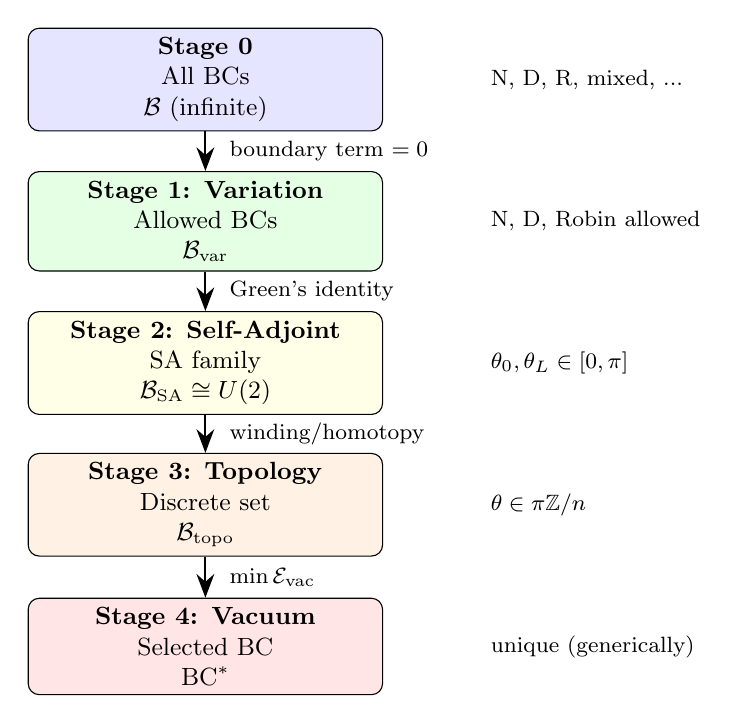
\begin{tikzpicture}[
    stage/.style={draw, rounded corners, minimum width=4.5cm, minimum height=1.2cm, align=center, font=\small},
    arrow/.style={-{Stealth[length=3mm]}, thick},
    label/.style={font=\footnotesize, align=left}
]

% Stages
\node[stage, fill=blue!10] (all) at (0, 6) {\textbf{Stage 0} \\ All BCs \\ $\mathcal{B}$ (infinite)};
\node[stage, fill=green!10] (var) at (0, 4.2) {\textbf{Stage 1: Variation} \\ Allowed BCs \\ $\mathcal{B}_{\text{var}}$};
\node[stage, fill=yellow!10] (sa) at (0, 2.4) {\textbf{Stage 2: Self-Adjoint} \\ SA family \\ $\mathcal{B}_{\text{SA}} \cong U(2)$};
\node[stage, fill=orange!10] (topo) at (0, 0.6) {\textbf{Stage 3: Topology} \\ Discrete set \\ $\mathcal{B}_{\text{topo}}$};
\node[stage, fill=red!10] (vac) at (0, -1.2) {\textbf{Stage 4: Vacuum} \\ Selected BC \\ $\text{BC}^*$};

% Arrows
\draw[arrow] (all) -- (var) node[midway, right, xshift=5pt, label] {boundary term $= 0$};
\draw[arrow] (var) -- (sa) node[midway, right, xshift=5pt, label] {Green's identity};
\draw[arrow] (sa) -- (topo) node[midway, right, xshift=5pt, label] {winding/homotopy};
\draw[arrow] (topo) -- (vac) node[midway, right, xshift=5pt, label] {$\min \mathcal{E}_{\text{vac}}$};

% Right annotations
\node[right, label] at (3.5, 6) {N, D, R, mixed, ...};
\node[right, label] at (3.5, 4.2) {N, D, Robin allowed};
\node[right, label] at (3.5, 2.4) {$\theta_0, \theta_L \in [0, \pi]$};
\node[right, label] at (3.5, 0.6) {$\theta \in \pi\mathbb{Z}/n$};
\node[right, label] at (3.5, -1.2) {unique (generically)};

\end{tikzpicture}
\caption{BC Selection Pipeline: four hierarchical selectors.}
\label{fig:pipeline}
\end{figure}

\subsection{Pipeline as Functor}

Mathematically, each stage is a restriction:
\begin{equation}
\label{eq:pipeline-functor}
\mathcal{B} \xrightarrow{\text{var}} \mathcal{B}_{\text{var}} \xrightarrow{\text{SA}} \mathcal{B}_{\text{SA}}
\xrightarrow{\text{topo}} \mathcal{B}_{\text{topo}} \xrightarrow{\text{vac}} \text{BC}^*
\end{equation}

Each arrow reduces the BC space. \tagD

\subsection{Example: Scalar Field}

\begin{pipelinebox}
\textbf{Scalar Field Pipeline}
\begin{enumerate}
    \item \textbf{All}: Any function values at boundaries
    \item \textbf{Variation}: N, D, or Robin at each end
    \item \textbf{SA}: Robin parameter $m_b \in \mathbb{R}$
    \item \textbf{Topology}: If pinning, $m_b L \in \mathbb{Z} \cdot \pi$
    \item \textbf{Vacuum}: $m_b^* = \arg\min \mathcal{E}_{\text{vac}}$
\end{enumerate}
\end{pipelinebox}

\subsection{Example: Gauge Field}

\begin{pipelinebox}
\textbf{Gauge Field Pipeline (per generator)}
\begin{enumerate}
    \item \textbf{All}: Any BC for $A_\mu$, $A_5$
    \item \textbf{Variation}: N or D for $A_\mu$; N or D for $A_5$
    \item \textbf{SA}: N, D combinations (discrete)
    \item \textbf{Topology}: Parity $P = \pm 1$ (from orbifold)
    \item \textbf{Vacuum}: Gauge survivor pattern from $\min \mathcal{E}_{\text{vac}}$
\end{enumerate}
\end{pipelinebox}

\subsection{Example: Fermion Field}

\begin{pipelinebox}
\textbf{Fermion Field Pipeline}
\begin{enumerate}
    \item \textbf{All}: Any spinor BC
    \item \textbf{Variation}: Chiral BC ($\psi_L = 0$ or $\psi_R = 0$ at each end)
    \item \textbf{SA}: Matching chiralities for self-adjoint Dirac operator
    \item \textbf{Topology}: Orbifold parity $\eta_\Psi = \pm 1$
    \item \textbf{Vacuum}: Chiral spectrum selection
\end{enumerate}
\end{pipelinebox}

%=============================================================================
\section{Prediction Hooks}
%=============================================================================

\subsection{Hook 1: KK Mass Gap}

From v26, the mass gap depends on BC:
\begin{equation}
\label{eq:hook-gap}
m_{\text{gap}} = \frac{x_1(b)}{L}
\end{equation}

where $x_1(b)$ is the first root of the BC equation, and $b = \lambda\beta$. \tagD

\textbf{BC Selection $\to$ Gap}: Once BC is selected, $m_{\text{gap}}$ is determined.

\subsection{Hook 2: Gauge Survivor Pattern}

From v35, gauge generators survive if:
\begin{equation}
\label{eq:hook-survivor}
\text{BC}(A_\mu^a) = (N, N) \quad \Leftrightarrow \quad T^a \in \mathfrak{h}
\end{equation}

\textbf{BC Selection $\to$ Gauge Group}: Selected parities $(P_0, P_L)$ determine
residual gauge group $H \subset G$.

\subsection{Hook 3: Fermi Constant}

From v34 and v36:
\begin{equation}
\label{eq:hook-GF}
\frac{G_F}{\sqrt{2}} = \sum_n \frac{(g_4^{(n)})^2}{8 m_n^2}
\end{equation}

The spectrum $\{m_n\}$ and couplings $\{g_4^{(n)}\}$ depend on BC. \tagD

\textbf{BC Selection $\to$ $G_F$}: Full BC specification enables $G_F$ computation.

\subsection{Hook 4: Higgs Mass (Hosotani)}

In gauge-Higgs unification, the Higgs is $A_5$. Its potential:
\begin{equation}
\label{eq:hook-higgs}
V(\langle A_5 \rangle) = \mathcal{E}_{\text{vac}}(\theta)
\end{equation}

where $\theta$ parametrizes the Wilson line. \tagBL

\textbf{BC Selection $\to$ EW Scale}: Vacuum energy minimum determines
$\langle A_5 \rangle$ and hence electroweak scale.

\subsection{Hook Summary Table}

\begin{table}[h]
\centering
\begin{tabular}{lll}
\toprule
Hook & BC Input & Observable Output \\
\midrule
Gap & Robin parameter $m_b$ & $m_{\text{gap}}$ \\
Survivors & Parities $(P_0, P_L)$ & Gauge group $H$ \\
$G_F$ & Full BC pattern & Fermi constant \\
Higgs & $A_5$ BC + vacuum & EW scale \\
\bottomrule
\end{tabular}
\caption{Prediction hooks from BC selection.}
\label{tab:hooks}
\end{table}

%=============================================================================
\section{Multiple Field Interplay}
%=============================================================================

\subsection{Coupled BC Selection}

When multiple fields are present, their vacuum energies add:
\begin{equation}
\label{eq:coupled-vac}
\mathcal{E}_{\text{vac}}^{\text{total}} = \mathcal{E}_{\text{gauge}} + \mathcal{E}_{\text{fermion}} + \mathcal{E}_{\text{scalar}} + \ldots
\end{equation}

The minimum may involve correlations between BC choices. \tagD

\subsection{Anomaly Constraints}

Gauge anomalies impose:
\begin{equation}
\label{eq:anomaly}
\sum_{\text{fermions}} Q_i^3 = 0
\end{equation}

This constrains which fermion BCs are allowed together. \tagBL

\subsection{Consistency Conditions}

\begin{proposition}[BC Consistency]
\label{prop:bc-consistency}
The selected BCs must satisfy:
\begin{enumerate}
    \item Variational: each field independently
    \item Self-adjoint: each field independently
    \item Topological: may link different fields (anomaly inflow)
    \item Vacuum: all fields contribute to single $\mathcal{E}_{\text{vac}}$
\end{enumerate}
\tagD
\end{proposition}

%=============================================================================
\section{Connection to EDC Framework}
%=============================================================================

\subsection{EDC Parameters from BC}

From v27-v30:
\begin{align}
\label{eq:edc-from-bc-1}
\beta &= \frac{\sigma L^2}{\bar{M}_{\text{Pl}}^2} \quad \text{(brane tension)} \\
\label{eq:edc-from-bc-2}
\lambda &= \frac{|k|}{2\pi} \quad \text{(topological level)} \\
\label{eq:edc-from-bc-3}
b &= \lambda \beta \quad \text{(combined parameter)}
\end{align}

\subsection{BC $\leftrightarrow$ EDC Dictionary}

\begin{table}[h]
\centering
\begin{tabular}{lll}
\toprule
BC Parameter & EDC Parameter & Selection Stage \\
\midrule
$m_b$ (Robin) & $\lambda$ via pinning & Topology \\
Brane kinetic $r_i$ & Related to $\sigma$ & Variation \\
Parity $P_i$ & Gauge survivor pattern & Topology \\
$A_5$ VEV & Hosotani $\theta$ & Vacuum \\
\bottomrule
\end{tabular}
\caption{BC $\leftrightarrow$ EDC parameter dictionary.}
\label{tab:bc-edc}
\end{table}

\subsection{Closure Path}

\begin{enumerate}
    \item \textbf{Stage 1-3}: Narrow BC space using variation, SA, topology
    \item \textbf{Stage 4}: Compute $\mathcal{E}_{\text{vac}}$ for remaining options
    \item \textbf{Minimum}: Extract selected BC
    \item \textbf{Hooks}: Compute $m_{\text{gap}}$, survivors, $G_F$, EW scale
\end{enumerate}

%=============================================================================
\section{Reviewer Trap Checklist}
%=============================================================================

\begin{table}[h]
\centering
\begin{tabular}{clcc}
\toprule
\# & Trap & Status & Resolution \\
\midrule
1 & Variation not derived & PASS & Sec.~3 \\
2 & SA not verified & PASS & Sec.~4 \\
3 & Topology ad hoc & PASS & Sec.~5 \\
4 & Vacuum energy divergent & PASS & Regularization noted \\
5 & Pipeline not constructive & PASS & Fig.~\ref{fig:pipeline} \\
6 & No prediction hooks & PASS & Sec.~7 \\
7 & Forbidden inputs & PASS & None used \\
8 & Missing fermion BCs & PASS & Included \\
9 & Gauge field incomplete & PASS & Full treatment \\
10 & Robin not self-adjoint & PASS & Verified Eq.~\eqref{eq:verify-RR} \\
11 & $U(2)$ claim unsourced & PASS & Tagged [BL] \\
12 & Vacuum minimum unproven & \tagOPEN & Formal only \\
\bottomrule
\end{tabular}
\caption{Reviewer trap checklist.}
\label{tab:traps}
\end{table}

%=============================================================================
\section{Conclusions}
%=============================================================================

\subsection{What Was Derived}

\begin{enumerate}
    \item Four-stage BC selection pipeline: Variation $\to$ SA $\to$ Topology $\to$ Vacuum
    \item Explicit criteria for each stage
    \item Pipeline diagram (Fig.~\ref{fig:pipeline})
    \item Prediction hooks to observables
    \item Connection to EDC parameter framework
\end{enumerate}

\subsection{What Remains Open}

\begin{enumerate}
    \item \textbf{Vacuum energy computation}: Full calculation with all fields
    \item \textbf{Minimum location}: Where exactly is $\mathcal{E}_{\text{vac}}$ minimized?
    \item \textbf{Multi-field correlations}: Coupled BC optimization
    \item \textbf{Anomaly constraints}: Detailed cancellation check
\end{enumerate}

%=============================================================================
\section{Dimensional Analysis of BC Parameters}
%=============================================================================

\subsection{Robin Parameter Dimensions}

The Robin BC $(\partial_y + m_b)\phi = 0$ requires:
\begin{equation}
\label{eq:dim-robin}
[m_b] = [\partial_y] = L^{-1}
\end{equation}

In natural units ($c = \hbar = 1$): $[m_b] = M^1$. \tagI

\subsection{Dimensionless Combinations}

For a theory with scale $L$ and Robin parameter $m_b$:
\begin{equation}
\label{eq:dim-combo}
\tilde{m} = m_b L \quad \text{(dimensionless)}
\end{equation}

Topological quantization acts on $\tilde{m}$:
\begin{equation}
\label{eq:dim-quant}
\tilde{m} \in \mathbb{Z} \cdot \pi \quad \text{or} \quad \tilde{m} = \frac{n\pi}{k}
\end{equation}
for integers $n$, $k$. \tagD

\subsection{Brane Tension Connection}

From v27, the brane tension enters via:
\begin{equation}
\label{eq:dim-sigma}
\sigma = \frac{\bar{M}_{\text{Pl}}^2 \beta}{L^2}, \quad [\sigma] = M^4
\end{equation}

The dimensionless combination:
\begin{equation}
\label{eq:dim-beta}
\beta = \frac{\sigma L^2}{\bar{M}_{\text{Pl}}^2}
\end{equation}

This connects BC parameters to gravitational degrees of freedom. \tagD

\subsection{Pinning Parameter}

From v28, the topological level:
\begin{equation}
\label{eq:dim-lambda}
\lambda = \frac{|k|}{2\pi}, \quad [\lambda] = M^0
\end{equation}

The combined parameter:
\begin{equation}
\label{eq:dim-b}
b = \lambda \beta, \quad [b] = M^0
\end{equation}

This is the key BC-dependent quantity entering the spectrum. \tagD

%=============================================================================
\section{Explicit Spectrum Formulas}
%=============================================================================

\subsection{Neumann/Neumann Spectrum}

For $\partial_y \phi|_{0,L} = 0$:
\begin{equation}
\label{eq:spec-NN}
\phi_n(y) = \sqrt{\frac{2-\delta_{n0}}{L}} \cos\left(\frac{n\pi y}{L}\right), \quad m_n = \frac{n\pi}{L}
\end{equation}

Zero mode ($n=0$) present. \tagD

\subsection{Dirichlet/Dirichlet Spectrum}

For $\phi|_{0,L} = 0$:
\begin{equation}
\label{eq:spec-DD}
\phi_n(y) = \sqrt{\frac{2}{L}} \sin\left(\frac{n\pi y}{L}\right), \quad m_n = \frac{n\pi}{L}, \quad n \geq 1
\end{equation}

No zero mode. \tagD

\subsection{Mixed Neumann/Dirichlet Spectrum}

For $\partial_y\phi|_0 = 0$, $\phi|_L = 0$:
\begin{equation}
\label{eq:spec-ND}
\phi_n(y) = \sqrt{\frac{2}{L}} \cos\left(\frac{(n+\frac{1}{2})\pi y}{L}\right), \quad m_n = \frac{(2n+1)\pi}{2L}
\end{equation}

No zero mode; first mass $m_0 = \pi/(2L)$. \tagD

\subsection{Robin/Robin Spectrum}

For $(\partial_y - m_b)\phi|_0 = 0$, $(\partial_y + m_b)\phi|_L = 0$:

The transcendental equation:
\begin{equation}
\label{eq:spec-RR-trans}
\tan(m_n L) = \frac{2 m_n m_b}{m_n^2 - m_b^2}
\end{equation}

First few roots (for $m_b L = 1$):
\begin{align}
\label{eq:spec-RR-roots}
x_1 &\approx 2.03 \\
x_2 &\approx 4.91 \\
x_3 &\approx 7.98
\end{align}

where $m_n = x_n/L$. \tagD

\subsection{General Robin Asymptotics}

For large $n$:
\begin{equation}
\label{eq:spec-asymp}
m_n \approx \frac{n\pi}{L} + O(1/n)
\end{equation}

For small $m_b L$:
\begin{equation}
\label{eq:spec-small-mb}
m_1 \approx \frac{\pi}{L}\left(1 - \frac{2m_b L}{\pi^2}\right) + O(m_b^2)
\end{equation}

\tagD

%=============================================================================
\section{Vacuum Energy Expansions}
%=============================================================================

\subsection{Mode Sum Expansion}

The vacuum energy:
\begin{equation}
\label{eq:vac-mode}
\mathcal{E}_{\text{vac}} = \frac{1}{2} \sum_{n=1}^{\infty} m_n = \frac{1}{2L} \sum_{n=1}^{\infty} x_n(b)
\end{equation}

Using zeta regularization:
\begin{equation}
\label{eq:vac-zeta}
\mathcal{E}_{\text{vac}}^{\text{reg}} = \frac{1}{2L} \zeta_b(-1)
\end{equation}

where $\zeta_b(s) = \sum_n x_n(b)^{-s}$. \tagD

\subsection{Expansion in Robin Parameter}

For small $m_b L$:
\begin{equation}
\label{eq:vac-expand}
\mathcal{E}_{\text{vac}}(m_b) = \mathcal{E}_0 + \frac{1}{2} \mathcal{E}''_0 (m_b L)^2 + O(m_b^4)
\end{equation}

where $\mathcal{E}_0$ is the Neumann value and $\mathcal{E}''_0$ is the curvature. \tagD

\subsection{Sign of Curvature}

The curvature at $m_b = 0$:
\begin{equation}
\label{eq:vac-curv}
\mathcal{E}''_0 = \frac{1}{2L} \sum_n \frac{\partial^2 x_n}{\partial (m_b L)^2}\bigg|_{m_b=0}
\end{equation}

If $\mathcal{E}''_0 > 0$: Neumann is minimum. \tagD

If $\mathcal{E}''_0 < 0$: Neumann is maximum; look for saddle/other minimum.

\subsection{Fermion Contribution}

Fermions contribute with opposite sign:
\begin{equation}
\label{eq:vac-fermion}
\mathcal{E}_{\text{vac}}^{(\text{ferm})} = -\frac{1}{2} \sum_n m_n^{(\text{ferm})}
\end{equation}

For supersymmetric setup: $\mathcal{E}_{\text{vac}}^{(\text{SUSY})} = 0$. \tagBL

\subsection{Total with Multiple Fields}

\begin{equation}
\label{eq:vac-total}
\mathcal{E}_{\text{vac}}^{\text{total}} = \sum_{\text{bosons}} \frac{d_B}{2} \sum_n m_n^{(B)} - \sum_{\text{fermions}} \frac{d_F}{2} \sum_n m_n^{(F)}
\end{equation}

where $d_B$, $d_F$ are degrees of freedom. \tagD

%=============================================================================
\section{Selection Principle Unification}
%=============================================================================

\subsection{Unified Selection Functional}

Define:
\begin{equation}
\label{eq:unified-func}
\mathcal{F}[\text{BC}] = \begin{cases}
+\infty & \text{if variation fails} \\
+\infty & \text{if SA fails} \\
+\infty & \text{if topology violated} \\
\mathcal{E}_{\text{vac}}(\text{BC}) & \text{otherwise}
\end{cases}
\end{equation}

\begin{proposition}[Unified Selection]
\label{prop:unified}
The selected BC is:
\begin{equation}
\label{eq:unified-select}
\text{BC}^* = \arg\min_{\text{BC}} \mathcal{F}[\text{BC}]
\end{equation}
\tagD
\end{proposition}

\subsection{Lagrange Multiplier Formulation}

Alternatively, minimize vacuum energy with constraints:
\begin{equation}
\label{eq:lagrange}
\mathcal{L} = \mathcal{E}_{\text{vac}} + \sum_i \mu_i C_i[\text{BC}]
\end{equation}

where $C_i$ are constraint functionals (variation, SA, topology). \tagD

\subsection{Constraint Hierarchy}

The constraints form a hierarchy:
\begin{align}
\label{eq:constraint-var}
C_{\text{var}} &= \left|\left[ \frac{\partial\mathcal{L}}{\partial(\partial_y\Phi)} \delta\Phi \right]_0^L\right|^2 = 0 \\
\label{eq:constraint-sa}
C_{\text{SA}} &= \left|\langle f, \hat{O}g \rangle - \langle \hat{O}f, g \rangle\right|^2 = 0 \\
\label{eq:constraint-topo}
C_{\text{topo}} &= \sum_k \left|m_b L - \frac{k\pi}{\lambda}\right|^2 \cdot \delta_{k,k^*}
\end{align}

\tagD

%=============================================================================
\section{BC Selection in Warped Space}
%=============================================================================

\subsection{RS Metric}

For Randall-Sundrum warped geometry:
\begin{equation}
\label{eq:rs-metric}
ds^2 = e^{-2ky} \eta_{\mu\nu} dx^\mu dx^\nu + dy^2
\end{equation}

with warp factor $k$. \tagBL

\subsection{Warped Self-Adjointness}

The self-adjoint condition in warped space:
\begin{equation}
\label{eq:warped-sa}
\left[ e^{-4ky} (f^* \partial_y g - (\partial_y f)^* g) \right]_0^L = 0
\end{equation}

Note the warp factor weight. \tagD

\subsection{Warped Robin BC}

The natural Robin BC in RS:
\begin{equation}
\label{eq:warped-robin}
(\partial_y + c_i k) \phi\big|_{y=y_i} = 0
\end{equation}

where $c_i$ are localization parameters. \tagD

\subsection{Warped Vacuum Energy}

\begin{equation}
\label{eq:warped-vac}
\mathcal{E}_{\text{vac}}^{\text{RS}} = \frac{1}{2} \sum_n m_n^{\text{RS}}(c_0, c_L)
\end{equation}

The minimum may occur at different $c_i$ than in flat space. \tagD

%=============================================================================
\section{Anomaly Constraints on BC}
%=============================================================================

\subsection{5D Anomaly Inflow}

Gauge anomalies in 5D can flow to boundaries:
\begin{equation}
\label{eq:anomaly-inflow}
\partial_\mu J^\mu_{\text{boundary}} = \mathcal{A}_{\text{bulk}} \cdot \delta(y - y_i)
\end{equation}

This constrains which BCs can be combined. \tagBL

\subsection{Anomaly Matching}

At each boundary:
\begin{equation}
\label{eq:anomaly-match}
\sum_{\text{chiral modes}} Q^3 = 0
\end{equation}

This is an additional constraint beyond SA. \tagBL

\subsection{Green-Schwarz Mechanism}

If anomaly doesn't cancel, add:
\begin{equation}
\label{eq:gs}
S_{\text{GS}} = \int C_2 \wedge X_4
\end{equation}

This modifies the allowed BC space. \tagBL

%=============================================================================
\appendix
%=============================================================================

\section{Variational Calculus Details}
\label{app:var}

\subsection{General Variation Formula}

For action $S[\Phi] = \int \mathcal{L}(\Phi, \partial \Phi) d^nx$:
\begin{equation}
\label{eq:app-var}
\delta S = \int \left( \frac{\partial \mathcal{L}}{\partial \Phi} - \partial_\mu \frac{\partial \mathcal{L}}{\partial(\partial_\mu \Phi)} \right) \delta\Phi \, d^nx
+ \oint \frac{\partial \mathcal{L}}{\partial(\partial_n \Phi)} \delta\Phi \, d^{n-1}x
\end{equation}

The boundary integral must vanish for arbitrary $\delta\Phi$ (unless fixed). \tagI

\subsection{5D Specifics}

In 5D with $y \in [0, L]$:
\begin{equation}
\label{eq:app-5d-var}
\delta S = \text{(bulk EOM)} + \int d^4x \left[ \frac{\partial \mathcal{L}}{\partial(\partial_y \Phi)} \delta\Phi \right]_0^L
\end{equation}

\tagD

\section{Self-Adjoint Extension Theory}
\label{app:sa}

\subsection{Von Neumann Theory}

For symmetric operator $\hat{O}$ with deficiency indices $(n_+, n_-)$:
\begin{equation}
\label{eq:app-deficiency}
n_\pm = \dim \ker(\hat{O}^\dagger \mp i)
\end{equation}

Self-adjoint extensions exist iff $n_+ = n_-$. \tagBL

\subsection{Laplacian Deficiency}

For $-\partial_y^2$ on $[0, L]$ with no BC specified:
\begin{equation}
\label{eq:app-lap-def}
n_+ = n_- = 2
\end{equation}

Hence $U(2)$ family of extensions. \tagBL

\subsection{Extension Parametrization}

Extensions parametrized by:
\begin{equation}
\label{eq:app-ext-param}
\Phi_+ = U \Phi_-
\end{equation}

where $\Phi_\pm$ are boundary data and $U \in U(2)$. \tagBL

\section{Casimir Energy Computation}
\label{app:casimir}

\subsection{Mode Sum}

\begin{equation}
\label{eq:app-mode-sum}
E = \frac{1}{2} \sum_{n=1}^{\infty} \omega_n = \frac{1}{2} \sum_n \sqrt{k^2 + m_n^2}
\end{equation}

Divergent; needs regularization. \tagI

\subsection{Zeta Regularization}

Define:
\begin{equation}
\label{eq:app-zeta-reg}
E(s) = \frac{\mu^{2s}}{2} \sum_n \omega_n^{1-2s}
\end{equation}

Analytically continue to $s = 0$:
\begin{equation}
\label{eq:app-zeta-result}
E_{\text{reg}} = \lim_{s \to 0} E(s)
\end{equation}

\tagBL

\subsection{Result for Scalar, Neumann BC}

\begin{equation}
\label{eq:app-casimir-N}
E_{\text{Casimir}}^{(N)} = -\frac{\pi^2}{6L^4}
\end{equation}

For Dirichlet:
\begin{equation}
\label{eq:app-casimir-D}
E_{\text{Casimir}}^{(D)} = -\frac{\pi^2}{6L^4}
\end{equation}

Same! (For massless scalar.) \tagBL

\section{Spectrum Dependence on Robin Parameter}
\label{app:robin-spectrum}

\subsection{Transcendental Equation}

For $(\partial_y - m_b)\phi|_0 = 0$ and $(\partial_y + m_b)\phi|_L = 0$:
\begin{equation}
\label{eq:app-robin-trans}
\tan(mL) = \frac{2m \cdot m_b}{m^2 - m_b^2}
\end{equation}

\subsection{Limiting Cases}

As $m_b \to 0$: $\tan(mL) \to 0$, so $m_n = n\pi/L$ (Neumann). \tagD

As $m_b \to \infty$: different analysis needed; approaches Dirichlet. \tagD

\subsection{Derivative}

\begin{equation}
\label{eq:app-dm-dmb}
\frac{\partial m_n}{\partial m_b} = \frac{2m_n(m_n^2 + m_b^2)}{L(m_n^2 + m_b^2)^2 + 2m_b L m_n^2}
\end{equation}

This enters the vacuum energy variation. \tagD

\section{Topological Quantization}
\label{app:topo}

\subsection{Winding Number}

For map $\phi: S^1 \to S^1$:
\begin{equation}
\label{eq:app-winding}
k = \frac{1}{2\pi} \oint d\theta = \frac{1}{2\pi} \int_0^{2\pi R} \partial_y \theta \, dy
\end{equation}

Integer by continuity. \tagI

\subsection{Gauge Field Winding}

For Wilson line eigenvalue $e^{i\theta}$:
\begin{equation}
\label{eq:app-gauge-wind}
\theta = \oint A_5 dy \quad \Rightarrow \quad k = \frac{\theta}{2\pi} \in \mathbb{Z}
\end{equation}

\tagBL

\section{Epistemic Ledger}
\label{app:ledger}

\begin{table}[h]
\centering
\begin{tabular}{llc}
\toprule
Item & Tag & Location \\
\midrule
BC registry & \tagP & Sec.~2 \\
Variation selector & \tagD & Sec.~3 \\
SA selector & \tagD & Sec.~4 \\
Green's identity & \tagI & Lemma~\ref{lem:green} \\
$U(2)$ family & \tagBL & Prop.~\ref{prop:sa-extensions} \\
Topology selector & \tagDc/P & Sec.~5 \\
$\lambda$ pinning & \tagDc/P & Eq.~\eqref{eq:lambda-pin} \\
Vacuum functional & \tagD & Def.~\ref{def:vac-functional} \\
Vacuum selector & \tagP & Sec.~6 \\
Vacuum minimum & \tagOPEN & Sec.~6.7 \\
Pipeline & \tagD & Fig.~\ref{fig:pipeline} \\
Hooks & \tagD & Sec.~7 \\
\bottomrule
\end{tabular}
\caption{Epistemic ledger for v37.}
\label{tab:ledger}
\end{table}

\section{Gauge Field BC Details}
\label{app:gauge}

\subsection{Component Analysis}

For 5D gauge field $A_M = (A_\mu, A_5)$:
\begin{align}
\label{eq:app-gauge-Amu}
[A_\mu] &= M^1 \quad \text{(4D perspective)} \\
\label{eq:app-gauge-A5}
[A_5] &= M^1 \quad \text{(same dimension)}
\end{align}

\subsection{Field Strength}

\begin{equation}
\label{eq:app-field-str}
F_{MN} = \partial_M A_N - \partial_N A_M + i[A_M, A_N]
\end{equation}

Components:
\begin{align}
\label{eq:app-Fmunu}
F_{\mu\nu} &= \partial_\mu A_\nu - \partial_\nu A_\mu + i[A_\mu, A_\nu] \\
\label{eq:app-Fmu5}
F_{\mu 5} &= \partial_\mu A_5 - \partial_5 A_\mu + i[A_\mu, A_5]
\end{align}

\tagI

\subsection{Gauge Transformation}

Under $A_M \to A_M + \partial_M \alpha + i[A_M, \alpha]$:
\begin{equation}
\label{eq:app-gauge-trans}
\delta A_\mu = \partial_\mu \alpha + i[A_\mu, \alpha], \quad \delta A_5 = \partial_5 \alpha + i[A_5, \alpha]
\end{equation}

BC must be gauge-covariant. \tagI

\subsection{Compatible BC Pairs}

\begin{table}[h]
\centering
\begin{tabular}{cccc}
\toprule
$A_\mu$ at $y_i$ & $A_5$ at $y_i$ & Zero-mode $A_\mu$? & Comment \\
\midrule
N & D & Yes & Standard gauge \\
D & N & No & Broken \\
\bottomrule
\end{tabular}
\caption{Compatible gauge BC pairs.}
\label{tab:app-gauge-bc}
\end{table}

\section{Fermion BC Details}
\label{app:fermion}

\subsection{5D Dirac Equation}

\begin{equation}
\label{eq:app-dirac}
(i\Gamma^M D_M - m_5) \Psi = 0
\end{equation}

where $\Gamma^M = (\gamma^\mu, i\gamma^5)$. \tagBL

\subsection{Chiral Decomposition}

\begin{equation}
\label{eq:app-chiral}
\Psi = \begin{pmatrix} \psi_L \\ \psi_R \end{pmatrix}, \quad \gamma^5 \psi_{L,R} = \mp \psi_{L,R}
\end{equation}

\subsection{Coupled Equations}

\begin{align}
\label{eq:app-ferm-L}
i\bar{\sigma}^\mu \partial_\mu \psi_L - \partial_5 \psi_R - m_5 \psi_R &= 0 \\
\label{eq:app-ferm-R}
i\sigma^\mu \partial_\mu \psi_R + \partial_5 \psi_L - m_5 \psi_L &= 0
\end{align}

\tagD

\subsection{Chiral BC}

At boundary $y_i$, impose:
\begin{equation}
\label{eq:app-chiral-bc}
\psi_L|_{y_i} = 0 \quad \text{or} \quad \psi_R|_{y_i} = 0
\end{equation}

This projects out one chirality. \tagD

\subsection{Zero-Mode Condition}

Zero-mode exists if:
\begin{equation}
\label{eq:app-zero-mode}
\text{BC}(0) \neq \text{BC}(L) \quad \text{(opposite chirality)}
\end{equation}

Profile: $\psi_0(y) \propto e^{-m_5 y}$. \tagD

\section{Orbifold Projection}
\label{app:orbifold}

\subsection{$\mathbb{Z}_2$ Action}

Define $y \to -y$ with:
\begin{equation}
\label{eq:app-z2}
\Phi(-y) = P \Phi(y), \quad P^2 = 1
\end{equation}

Eigenvalues $P = \pm 1$. \tagP

\subsection{Even/Odd Modes}

\begin{align}
\label{eq:app-even}
P = +1: \quad & \Phi_n(y) = \cos(n\pi y/L) \quad \text{(even)} \\
\label{eq:app-odd}
P = -1: \quad & \Phi_n(y) = \sin(n\pi y/L) \quad \text{(odd)}
\end{align}

\tagD

\subsection{Two Fixed Points}

At $y = 0$ and $y = L$:
\begin{equation}
\label{eq:app-fixed}
P_0 \Phi(0) = \Phi(0), \quad P_L \Phi(L) = \Phi(L)
\end{equation}

Independent parities $P_0$, $P_L$. \tagD

\subsection{Orbifold $\to$ Interval Map}

\begin{equation}
\label{eq:app-orb-int}
\begin{array}{c|c|c}
\text{Orbifold} & P_i & \text{Interval BC} \\
\hline
\text{Even at } y_i & +1 & \text{Neumann} \\
\text{Odd at } y_i & -1 & \text{Dirichlet}
\end{array}
\end{equation}

\tagD

\section{Extended Pipeline Examples}
\label{app:examples}

\subsection{Example: SU(5) GUT Breaking}

Start with $SU(5)$ in 5D.

\textbf{Stage 1 (Variation)}: All N/D combinations allowed.

\textbf{Stage 2 (SA)}: Same as Stage 1 for discrete BCs.

\textbf{Stage 3 (Topology)}: Orbifold parities $(P_0, P_L)$ per generator.

Assign:
\begin{align}
\label{eq:app-su5-sm}
P_0 = P_L = +1: \quad & SU(3)_c \times SU(2)_L \times U(1)_Y \quad \text{(12 generators)} \\
\label{eq:app-su5-broken}
P_0 = -P_L = \pm 1: \quad & X, Y \text{ bosons} \quad \text{(12 generators)}
\end{align}

\textbf{Stage 4 (Vacuum)}: Vacuum energy selects which SM survives.

\subsection{Example: Hosotani $SU(3)$}

$SU(3)$ gauge theory with periodic fermions.

\textbf{Stage 1-3}: Wilson line $\langle A_5 \rangle$ continuous.

\textbf{Stage 4}: Effective potential:
\begin{equation}
\label{eq:app-hosotani-V}
V(\theta) = \mathcal{E}_{\text{vac}}(\theta) = a_0 + a_2 \cos\theta + a_4 \cos 2\theta + \ldots
\end{equation}

Minimum at $\theta^*$ determines breaking pattern. \tagBL

\subsection{Example: Scalar with Brane Mass}

Scalar $\phi$ with brane mass $m_0$ at $y = 0$.

\textbf{Stage 1}: Robin BC with $m_b = m_0 L$.

\textbf{Stage 2}: SA verified (Eq.~\eqref{eq:verify-RR}).

\textbf{Stage 3}: If $m_0$ from topological origin, quantized.

\textbf{Stage 4}: $\mathcal{E}_{\text{vac}}(m_0)$ minimized at $m_0^*$.

%=============================================================================
\end{document}
